\documentclass[11pt,a4paper]{article}
\usepackage[margin=21mm]{geometry}
\usepackage[T1]{fontenc}
\usepackage{lmodern,amsmath,amssymb,booktabs,array,tabularx}
\usepackage{xcolor,pgfplots,hyperref}
\pgfplotsset{compat=1.18}
\hypersetup{colorlinks=true,linkcolor=blue!50!black,citecolor=blue!50!black,urlcolor=blue!50!black}
\setlength{\parindent}{0pt}
\setlength{\parskip}{5pt}
\setlength{\emergencystretch}{2em}
\renewcommand{\arraystretch}{1.15}
\newcommand{\E}{\mathbb{E}}
\newcommand{\Var}{\operatorname{Var}}
\newcommand{\med}{\operatorname{median}}
\newcommand{\code}[1]{\texttt{\detokenize{#1}}}
\pgfplotsset{reportaxis/.style={width=\linewidth,height=6cm,
scale only axis=false,axis lines=left,grid=major,grid style={gray!15},
tick label style={font=\scriptsize},label style={font=\footnotesize},
title style={font=\small},xticklabel style={rotate=40,anchor=east},
legend style={font=\tiny,draw=none,fill=white,at={(.03,.97)},anchor=north west},
scaled y ticks=false,y tick label style={/pgf/number format/fixed},
unbounded coords=discard}}
\title{Graphical Replication Review\\[4pt]
\large Close Matches, Remaining Discrepancies, and Justified Assumptions}
\author{Jump-Diffusion Option Pricing Replication Project}
\date{4 October 2026}

\begin{document}
\maketitle
\vspace{-8mm}
\begin{abstract}
This report compares the current reconstruction with the graphs in
Volk-Makarewicz, Borovkova, and Heidergott~\cite{paper}. It begins with
the components showing the closest agreement, then examines the larger
price, rejection-probability, and power discrepancies. Each material
assumption is linked to evidence in the paper, a mathematical justification,
and its remaining limitation. The current implementation is internally
checked under an explicit specification. It is not a verified one-to-one
reproduction of every published curve.
\end{abstract}

\section{The closest matches and their small differences}
\subsection{Merton relative-price curves: the strongest agreement}
The lower panel of the paper's Figure~1(a), comparing GBM and Merton
call prices, is the strongest visual match. Both versions show a rising
relative price difference as $\rho=\lambda/\sigma$ increases, with the
$\lambda=0.01$ curve highest and the $\lambda=0.70$ curve lowest over
the displayed grid. The reconstructed curves have the same overall
scale and ordering. The analogous mean-price curves in the paper's
Figure~3(a) also show this qualitative agreement.

The most clearly recorded point is $\lambda=0.01$, $\rho=2$:
\begin{center}
\begin{tabular}{@{}lr@{}}
\toprule
Quantity & Relative price difference\\
\midrule
Paper Figure 1(a), visual reading & $\approx 0.058$\\
Current ratio of median price estimates & $0.057702$\\
Current ratio of mean price estimates & $0.057518$\\
\bottomrule
\end{tabular}
\end{center}
The median-based result differs from the approximate paper reading by
$0.000298$, or about $0.51\%$ of that reading. The mean-based result is
included to show the small effect of aggregation; it is not compared
as though it were the paper's median statistic.

\textbf{How far this agreement extends.} The lower Merton price panels
are visually close, and one median endpoint has a recorded numerical
comparison. A point-by-point numerical match of all Merton curves has
not been established. In particular, closeness of prices does not
establish closeness of the upper power panels.

\subsection{Why small differences can remain in these close panels}
The authors' random seed, random-number generator settings, and numerical
curve arrays are unavailable. Our sample medians and means therefore
need not equal theirs even when the model is the same. A value read
from a raster graph also has limited precision; $0.058$ is not an exact
author-supplied number. Small differences in sampling, finite outer
repetitions, and rounding are plausible explanations for the residual
Merton gap. They have not been individually identified or quantified
against the authors' experiment. Typography and interpolation between
markers can affect appearance but do not change the underlying prices.

\clearpage
\begin{figure}[ht]
\centering
\begin{minipage}[t]{.485\linewidth}
\centering
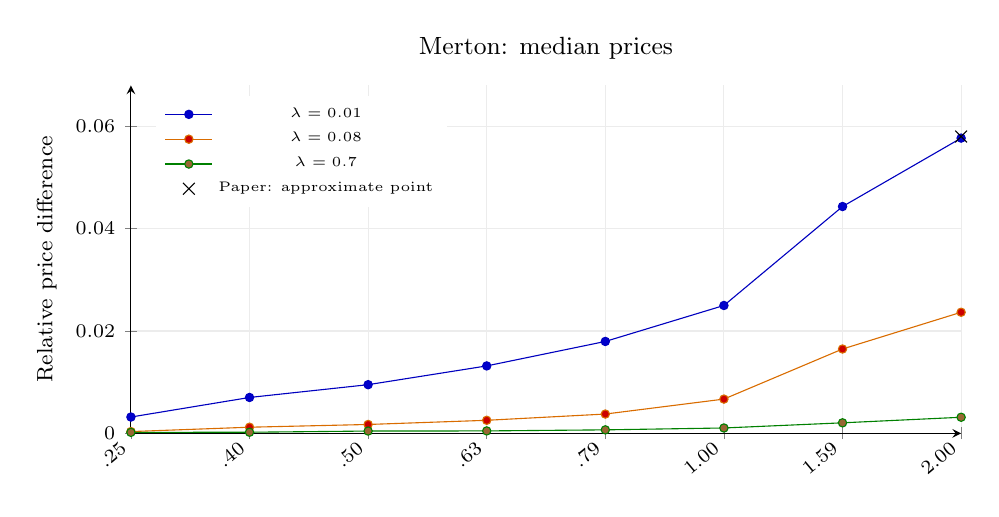
\begin{tikzpicture}
\begin{axis}[reportaxis,xmin=0,xmax=7,ymin=0,xtick={0,1,2,3,4,5,6,7},xticklabels={.25,.40,.50,.63,.79,1.00,1.59,2.00},ymax=0.068,title={Merton: median prices},ylabel={Relative price difference}]
\addplot+[color=blue!75!black,mark=*,mark size=1.5pt] coordinates {(0,0.003183746422) (1,0.007009491727) (2,0.009507512869) (3,0.01317569203) (4,0.01795759315) (5,0.0249898185) (6,0.04432856448) (7,0.05770218875)};
\addlegendentry{$\lambda=0.01$}
\addplot+[color=orange!85!black,mark=*,mark size=1.5pt] coordinates {(0,0.0003418355454) (1,0.001194532689) (2,0.001729992206) (3,0.002546222698) (4,0.003768897022) (5,0.006691112815) (6,0.01648080771) (7,0.02366384287)};
\addlegendentry{$\lambda=0.08$}
\addplot+[color=green!50!black,mark=*,mark size=1.5pt] coordinates {(0,0.0001863137853) (1,0.0002117735831) (2,0.0004448670122) (3,0.0004710932999) (4,0.0006790395601) (5,0.001045230233) (6,0.002053351869) (7,0.003139785801)};
\addlegendentry{$\lambda=0.7$}
\addplot+[only marks,color=black,mark=x,mark size=3pt] coordinates {(7,.058)};
\addlegendentry{Paper: approximate point}
\end{axis}
\end{tikzpicture}
\end{minipage}\hfill
\begin{minipage}[t]{.485\linewidth}
\centering
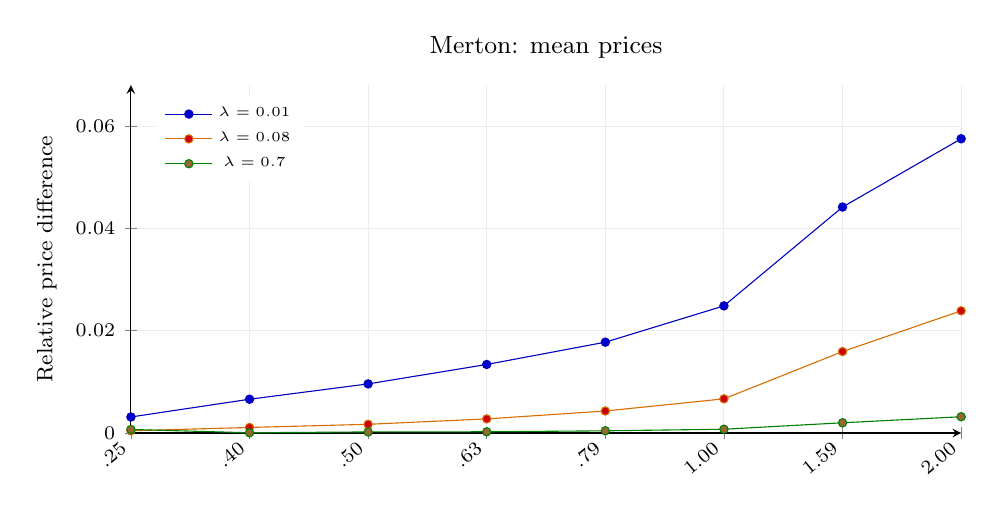
\begin{tikzpicture}
\begin{axis}[reportaxis,xmin=0,xmax=7,ymin=0,xtick={0,1,2,3,4,5,6,7},xticklabels={.25,.40,.50,.63,.79,1.00,1.59,2.00},ymax=0.068,title={Merton: mean prices},ylabel={Relative price difference}]
\addplot+[color=blue!75!black,mark=*,mark size=1.5pt] coordinates {(0,0.003140277461) (1,0.006610260129) (2,0.009604826954) (3,0.013404705) (4,0.01775856058) (5,0.02485728192) (6,0.04417342793) (7,0.05751848889)};
\addlegendentry{$\lambda=0.01$}
\addplot+[color=orange!85!black,mark=*,mark size=1.5pt] coordinates {(0,0.0004446861711) (1,0.001091682106) (2,0.00171016996) (3,0.002762363775) (4,0.004309213948) (5,0.006683355426) (6,0.01592608642) (7,0.02389226873)};
\addlegendentry{$\lambda=0.08$}
\addplot+[color=green!50!black,mark=*,mark size=1.5pt] coordinates {(0,0.0007003598297) (1,5.375980345e-05) (2,0.0002164278412) (3,0.0002471415576) (4,0.0004361609356) (5,0.0007466300693) (6,0.002007967236) (7,0.003185171002)};
\addlegendentry{$\lambda=0.7$}
\end{axis}
\end{tikzpicture}
\end{minipage}
\caption{Current Merton relative-price curves. Left: medians, corresponding
to the lower paper Figure 1(a). Right: means, corresponding to the lower
paper Figure 3(a). Horizontal ticks show $\lambda/\sigma$ and are spaced
categorically as in the source. The black cross is the approximate
Figure 1(a) endpoint only; it is not a digitized paper curve.}
\label{fig:close}
\end{figure}

\subsection{Other similarities are more limited}
At high jump intensity, the Merton rejection curve in Figure~2 remains
near the $0.10$ significance level in both the paper and the current
run. For example, current GradTwo rejection frequencies at
$\lambda=0.70$, $\rho=0.5$ are $0.094$ for 256 paths and $0.122$ for
16,384 paths. This is a similarity in rejection behavior, not evidence
that the corresponding power calculation matches.

For the MRJD cases, several rejection curves approach one as the path
count grows, as in the paper. However, they can reach that level much
later in our reconstruction. Agreement at the upper limit alone is
weak evidence: many different alternatives become detectable with
enough observations.

\section{What is being compared}
The reference is the supplied article~\cite{paper}, with printed pages
740--751. The supplied and project copies have identical extracted
page text and identical embedded Figures~1--3. Paper values quoted
from graphs below are approximate visual readings, not machine-readable
author data. Our plotted points come directly from the saved simulation
summaries; no curve has been adjusted to improve visual agreement.

Let $\widehat V_{P,r}$ and $\widehat V_{Q,r}$ be the diffusion and jump-model
price estimates in outer run $r$. The price statistics are
\begin{align}
R_{\mathrm{med}}&=
\frac{|\med_r\widehat V_{Q,r}-\med_r\widehat V_{P,r}|}
{|\med_r\widehat V_{P,r}|},\\
R_{\mathrm{mean}}&=
\frac{|\overline{\widehat V_Q}-\overline{\widehat V_P}|}
{|\overline{\widehat V_P}|}.
\end{align}
The first is a ratio of separately aggregated prices, not the median
of pathwise or runwise relative differences. Price records are counted
once per run, although each run produces three statistical-method rows.

\begin{center}\small
\begin{tabularx}{\linewidth}{@{}cXXX@{}}
\toprule
Paper figure & Horizontal axis & Upper panels & Lower panels\\
\midrule
1 & Model ratio & Median estimated power & $R_{\mathrm{med}}$\\
2 & Paths per estimate & Empirical rejection frequency & Median estimated power\\
3 & Same ratio grid as Figure 1 & Mean estimated power & $R_{\mathrm{mean}}$\\
\bottomrule
\end{tabularx}
\end{center}

\clearpage
\section{Price panels that do not match}
\subsection{Magnitude of the discrepancies}
\begin{center}\small
\begin{tabular}{@{}lrrrr@{}}
\toprule
Paper panel / contract & $\lambda$ & Ratio & Paper reading & Current $R_{\mathrm{med}}$\\
\midrule
a: Merton call & 0.01 & 2.00 & $\approx 0.058$ & 0.057702 \\
b: MRJD vanilla put & 0.70 & 0.67 & $\approx 0.8$ & 0.080431 \\
c: MRJD Asian call (4) & 0.70 & 1.00 & $\approx 0.37$ & 0.463874 \\
d: MRJD Asian put (12) & 0.70 & 0.67 & $\approx 5.2$ & 0.260139 \\
\bottomrule
\end{tabular}
\end{center}
Panel~(b) is compared at ratio $0.67$ because its high-intensity endpoint
at ratio 1 is clipped in the source figure. The panel~(d) marker at
ratio $0.67$ reads approximately 5.2; an earlier reading of 5.8 was
revised after inspecting the source image. These choices avoid treating
an axis limit or a clipped curve as an observed data point.

The vanilla-put discrepancy is approximately tenfold at the selected
point. The twelve-date discrepancy is approximately twentyfold. The
four-date Asian call is closer in scale, but its selected result is
about $25\%$ above the approximate paper reading. That is a material
discrepancy, not a close numerical replication.

\begin{figure}[ht]
\centering
\begin{minipage}[t]{.485\linewidth}
\centering
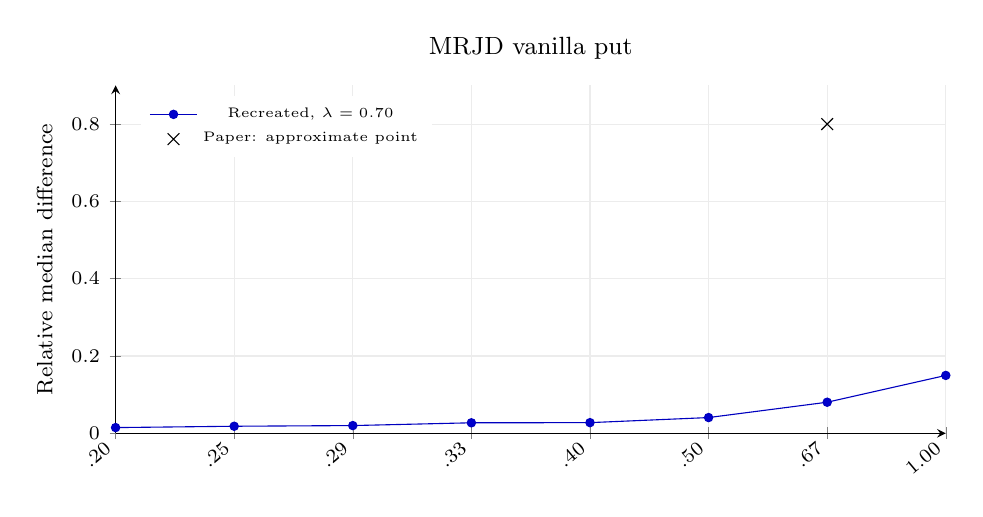
\begin{tikzpicture}
\begin{axis}[reportaxis,xmin=0,xmax=7,ymin=0,xtick={0,1,2,3,4,5,6,7},xticklabels={.20,.25,.29,.33,.40,.50,.67,1.00},ymax=0.9,title={MRJD vanilla put},ylabel={Relative median difference}]
\addplot+[blue!75!black,mark=*,mark size=1.5pt] coordinates {(0,0.01478585788) (1,0.01828349762) (2,0.02002760035) (3,0.02721058272) (4,0.02761893045) (5,0.04074850101) (6,0.08043074467) (7,0.1497585909)};
\addlegendentry{Recreated, $\lambda=0.70$}
\addplot+[only marks,color=black,mark=x,mark size=3pt] coordinates {(6,0.8)};
\addlegendentry{Paper: approximate point}
\end{axis}
\end{tikzpicture}
\end{minipage}\hfill
\begin{minipage}[t]{.485\linewidth}
\centering
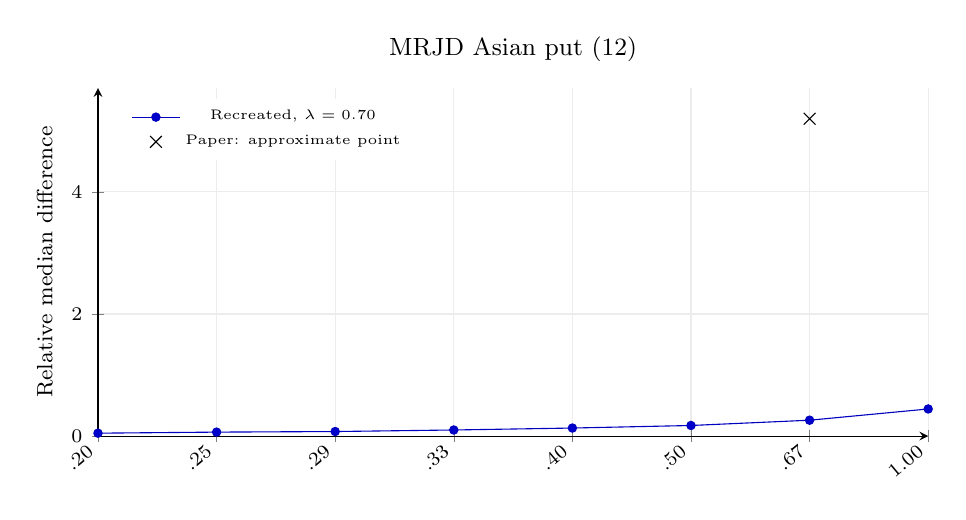
\begin{tikzpicture}
\begin{axis}[reportaxis,xmin=0,xmax=7,ymin=0,xtick={0,1,2,3,4,5,6,7},xticklabels={.20,.25,.29,.33,.40,.50,.67,1.00},ymax=5.7,title={MRJD Asian put (12)},ylabel={Relative median difference}]
\addplot+[blue!75!black,mark=*,mark size=1.5pt] coordinates {(0,0.0476732577) (1,0.06499044912) (2,0.07458193611) (3,0.0999283384) (4,0.131854611) (5,0.1735290304) (6,0.2601393791) (7,0.4443142366)};
\addlegendentry{Recreated, $\lambda=0.70$}
\addplot+[only marks,color=black,mark=x,mark size=3pt] coordinates {(6,5.2)};
\addlegendentry{Paper: approximate point}
\end{axis}
\end{tikzpicture}
\end{minipage}
\caption{Selected MRJD price discrepancies at $\lambda=0.70$. Blue curves
are current results; black crosses are individual approximate readings
from the paper. Horizontal ticks show $\E|J|/\sigma$. Each panel uses
one common vertical scale for its current curve and paper reference,
so the magnitude differences remain visible.}
\label{fig:mismatch}
\end{figure}

\subsection{Why changing GradOne or GradTwo cannot repair these panels}
The lower price panels use only the simulated $P$ and $Q$ payoffs.
They do not use the gradient estimator. Replacing randomized MVD with
exhaustive MVD can change standard errors, rejection rates, and estimated
power, but cannot change a price panel when the same $P/Q$ paths are used.
The large lower-panel gaps therefore point to the contract or model
specification, the parameter sweep, or another unidentified difference
in the original experiment. This is a diagnostic separation, not proof
that one particular ambiguity caused the discrepancy.

\clearpage
\section{Power and rejection graphs: a separate mismatch}
\subsection{Paper Figure 1: upper power panels}
The paper's MRJD gradient-power curves are mostly high across the ratio
grid. In our full run, at $\lambda=0.70$, median GradTwo power ranges
from about $0.195$ to $0.675$ for the vanilla put and $0.311$ to $0.890$
for the twelve-date put. The four-date call ranges from about $0.633$
to $0.993$: the endpoint is high, but the lower-ratio behavior differs.
The Merton price agreement also does not extend automatically to its
gradient-power curves. Differences concern the curve levels and shape,
not merely colors, line widths, or plot layout.

\subsection{Paper Figure 2: paths required to reject}
The source MRJD rejection curves rise to approximately one at comparatively
small path counts. Our curves often rise later. At 256 paths and
$\lambda=0.70$, the current GradTwo results are:
\begin{center}\small
\begin{tabular}{@{}lrr@{}}
\toprule
Contract & Rejection frequency & Median plug-in power\\
\midrule
Merton call & 0.0940 & 0.2090 \\
MRJD vanilla put & 0.1200 & 0.2153 \\
MRJD Asian call (4) & 0.7867 & 0.8499 \\
MRJD Asian put (12) & 0.4333 & 0.4624 \\
\bottomrule
\end{tabular}
\end{center}
The fixed ratios are $0.5$ for Merton and $0.33$ for MRJD. In the paper,
the MRJD GradTwo curves are visually near one around this part of the
path grid. The contrast is strongest for the vanilla put. The table
also illustrates why rejection frequency and estimated power must be
reported separately: they are not the same statistic.

\begin{figure}[ht]
\centering
\begin{minipage}[t]{.485\linewidth}
\centering
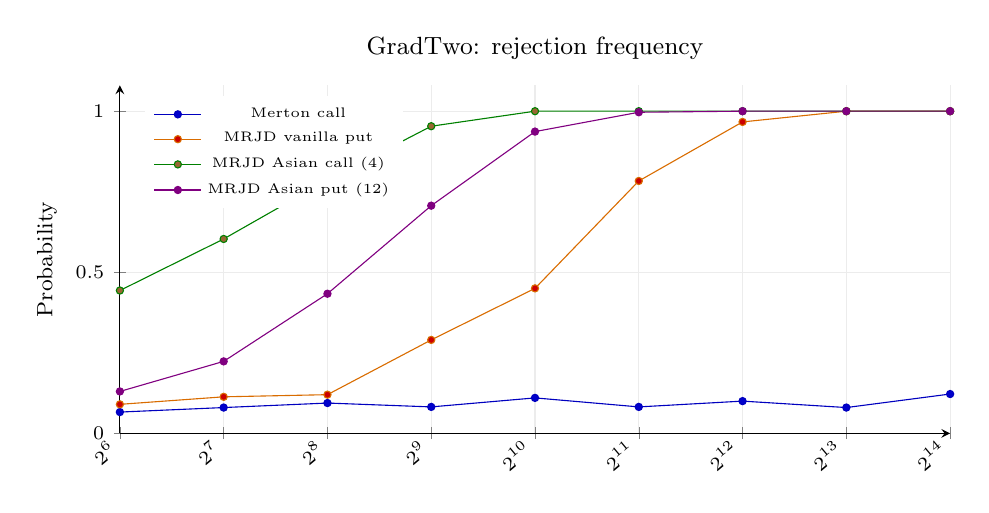
\begin{tikzpicture}
\begin{axis}[reportaxis,xmin=0,xmax=8,ymin=0,xtick={0,1,2,3,4,5,6,7,8},xticklabels={$2^{6}$,$2^{7}$,$2^{8}$,$2^{9}$,$2^{10}$,$2^{11}$,$2^{12}$,$2^{13}$,$2^{14}$},ymax=1.08,title={GradTwo: rejection frequency},ylabel={Probability}]
\addplot+[color=blue!75!black,mark=*,mark size=1.3pt] coordinates {(0,0.066) (1,0.08) (2,0.094) (3,0.082) (4,0.11) (5,0.082) (6,0.1) (7,0.08) (8,0.122)};
\addlegendentry{Merton call}
\addplot+[color=orange!85!black,mark=*,mark size=1.3pt] coordinates {(0,0.09) (1,0.1133333333) (2,0.12) (3,0.29) (4,0.45) (5,0.7833333333) (6,0.9666666667) (7,1) (8,1)};
\addlegendentry{MRJD vanilla put}
\addplot+[color=green!50!black,mark=*,mark size=1.3pt] coordinates {(0,0.4433333333) (1,0.6033333333) (2,0.7866666667) (3,0.9533333333) (4,1) (5,1) (6,1) (7,1) (8,1)};
\addlegendentry{MRJD Asian call (4)}
\addplot+[color=violet,mark=*,mark size=1.3pt] coordinates {(0,0.13) (1,0.2233333333) (2,0.4333333333) (3,0.7066666667) (4,0.9366666667) (5,0.9966666667) (6,1) (7,1) (8,1)};
\addlegendentry{MRJD Asian put (12)}
\end{axis}
\end{tikzpicture}
\end{minipage}\hfill
\begin{minipage}[t]{.485\linewidth}
\centering
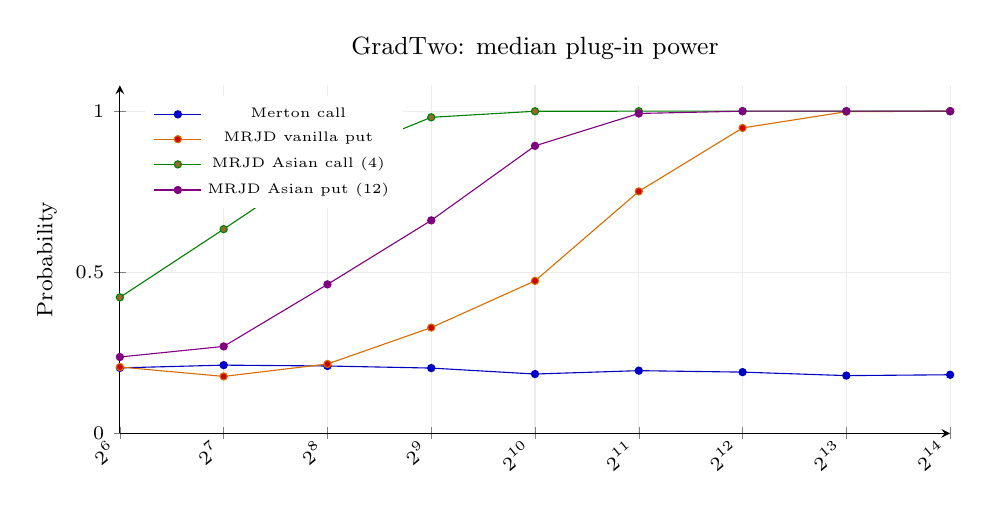
\begin{tikzpicture}
\begin{axis}[reportaxis,xmin=0,xmax=8,ymin=0,xtick={0,1,2,3,4,5,6,7,8},xticklabels={$2^{6}$,$2^{7}$,$2^{8}$,$2^{9}$,$2^{10}$,$2^{11}$,$2^{12}$,$2^{13}$,$2^{14}$},ymax=1.08,title={GradTwo: median plug-in power},ylabel={Probability}]
\addplot+[color=blue!75!black,mark=*,mark size=1.3pt] coordinates {(0,0.2031461498) (1,0.2116807649) (2,0.2090030939) (3,0.2025613717) (4,0.1840743504) (5,0.1945292357) (6,0.1899790512) (7,0.1791614464) (8,0.1818336275)};
\addlegendentry{Merton call}
\addplot+[color=orange!85!black,mark=*,mark size=1.3pt] coordinates {(0,0.2059318665) (1,0.176652333) (2,0.2152696018) (3,0.3282014534) (4,0.4732183751) (5,0.7510362543) (6,0.9479592677) (7,0.9984882713) (8,0.9999991787)};
\addlegendentry{MRJD vanilla put}
\addplot+[color=green!50!black,mark=*,mark size=1.3pt] coordinates {(0,0.4220652358) (1,0.6337728186) (2,0.8498829193) (3,0.9809652503) (4,0.9998286344) (5,0.9999999845) (6,1) (7,1) (8,1)};
\addlegendentry{MRJD Asian call (4)}
\addplot+[color=violet,mark=*,mark size=1.3pt] coordinates {(0,0.2369591655) (1,0.2697541652) (2,0.4623574119) (3,0.660993953) (4,0.8923859569) (5,0.9929364261) (6,0.9999887722) (7,1) (8,1)};
\addlegendentry{MRJD Asian put (12)}
\end{axis}
\end{tikzpicture}
\end{minipage}
\caption{Current Figure 2 quantities for GradTwo at $\lambda=0.70$.
Horizontal ticks are paths per estimate. These are reconstructed curves
only; no numerical paper power series was supplied. The legend identifies
contracts rather than the method/rate combinations used in the original.}
\end{figure}

\textbf{The four-run explanation no longer applies.} The present data
contain 500 outer runs per Merton setting and 300 per MRJD setting.
The earlier four-run output has been superseded and DEBUG is isolated.
Increasing the outer count improves estimation of the chosen experiment;
it cannot identify a missing model parameter or power algorithm.

\clearpage
\subsection{Paper Figure 3: replacing medians with means}
Figure~3 must reuse Figure~1's ratio experiment. The earlier implementation
incorrectly used the path-count experiment; that routing error is fixed.
At the same settings used in the price comparison table, the current
aggregation results are:
\begin{center}\small
\begin{tabular}{@{}lrr@{}}
\toprule
Contract & $R_{\mathrm{med}}$ & $R_{\mathrm{mean}}$\\
\midrule
Merton call & 0.057702 & 0.057518 \\
MRJD vanilla put & 0.080431 & 0.076972 \\
MRJD Asian call (4) & 0.463874 & 0.470299 \\
MRJD Asian put (12) & 0.260139 & 0.259373 \\
\bottomrule
\end{tabular}
\end{center}
The Merton price panel remains visually close under mean aggregation.
The large MRJD price gaps persist. Their scale is not explained by
choosing means instead of medians. Mean and median estimated power can
differ more because per-run power estimates may be skewed; changing
aggregation still does not recover the authors' unspecified calculation.

\section{Assumptions used to make the experiment well defined}
\subsection{MRJD ratio and preservation of the mean jump}
\textbf{Gap in the paper.} The figure axes use
$\rho=\E|J|/\sigma$, while Section~4, p.~747, gives
$\lambda/(\beta_+-\beta_-)$. Table~2 has $\beta_+=3.48$ and
$\beta_-=5.54$, so the latter denominator is $-2.06$ and the literal
ratio is negative. It cannot equal the positive plotted grid.
The same paragraph says the mean jump and sign probability remain
unchanged while the two directional magnitudes vary.

\textbf{Assumption and derivation.} We prioritize the plotted axis and
interpret ``mean jump'' as the signed mean $m_J=\E[J]$. With
$p=\Pr(J>0)=1/2$, the table implies $m_J=-1.03$. Writing
$a=\rho\sigma$, the constraints are
\[
p\beta_+-(1-p)\beta_-=m_J,\qquad
p\beta_++(1-p)\beta_-=a.
\]
They give the explicit mapping
\begin{equation}
\boxed{\beta_+=\frac{a+m_J}{2p},\qquad
\beta_-=\frac{a-m_J}{2(1-p)}}.
\end{equation}
Positive magnitudes require $a>|m_J|$. At $\sigma=5.16$, the feasibility
threshold is approximately $\rho>0.19961$; the configured grid begins
at $0.20$. The endpoint beta means are $(0.002,2.062)$ at ratio $0.20$
and $(4.13,6.19)$ at ratio 1.

\textbf{Justification and limit.} This satisfies the axis label and the
unchanged signed-mean statement simultaneously, whereas proportional
beta scaling changes the signed mean. The agreement with the grid's
lower boundary is a consistency observation, not evidence that the
authors used this exact mapping. The choice is explicit in configuration
and is not selected because it makes the curves look closer.

\clearpage
\subsection{Jump density, contract, and numerical parameters}
\textbf{Beta values are mean magnitudes.} The normalized numerical-study
density on p.~746 supports
\[
f_J(x)=\frac{p}{\beta_+}e^{-x/\beta_+}\mathbf{1}_{x>0}
+\frac{1-p}{\beta_-}e^{x/\beta_-}\mathbf{1}_{x<0},\qquad p=\tfrac12.
\]
This is stronger evidence than the nearby reversed sign-order sentence
or the generic density on p.~743, which omits a negative-side rate
multiplier. A reciprocal-beta interpretation remains a sensitivity
case rather than silently changing the distribution's units.

\textbf{Twelve-date payoff is a put.} Example~4, the study's prose,
and the in-panel headings specify a put; the subfigure captions say
call. We follow the formula and headings, evaluating
$e^{-rT}(K-A_{12})^+$ with $A_{12}=12^{-1}\sum_{j=1}^{12}S_{jT/12}$.
The call is priced separately. More pieces of internal evidence support
the put, but they do not prove which payoff generated the authors' files.

\textbf{Spot, strike, and monitoring dates follow explicit numbers.}
For MRJD, $S_0=40$, $K=35$, and $T=1$ are retained from Table~2.
Dates are $jT/m$, including maturity and excluding time zero.
The informal moneyness description is insufficient grounds for changing
the strike. Moneyness based on spot, terminal expectation, or an Asian
average need not give the same description under mean reversion.

\textbf{The unspecified diffusion risk adjustment is zero.} Equation~(8)
contains $\lambda^M$, but no numerical value is supplied. The baseline
sets it to zero and retains jump compensation:
\[
dX_t^Q=\bigl[\kappa(\theta-X_t^Q)-\lambda m_J\bigr]dt
+\sigma\,dW_t+dL_t,
\qquad L_t=\sum_{k=1}^{N_t}J_k.
\]
This is a transparent omission of an unprovided adjustment, not an
estimate of its true value. It is not calibrated against the paper's
graphs. Without author information, a nonzero value remains possible.

\textbf{Merton marks are normal in log space.} We use normal log marks
$Y$ and the compensator
$\lambda\E[e^Y-1]=\lambda(e^{\mu_J+s_J^2/2}-1)$.
The table value $\mu_J=-3.3\times10^{-5}$ is interpreted as the log-mark
mean. This is consistent with a lognormal multiplicative jump model,
but the paper also uses $\mu_J$ for drift in Eq.~(6). The close Merton
price point supports this reconstruction empirically; it does not
remove that notational ambiguity.

\subsection{What the alternative specifications establish}
Five explicit parameter interpretations, all three jump intensities,
all eight MRJD ratios, and four contracts were checked using independent
characteristic-function quadrature: 120 parameter settings and 480
expected-price comparisons. The complete parameter grid records both
beta magnitudes, signed and absolute moments, jump variance, volatility,
intensity, spot, strike, and maturity.

\begin{center}\small
\begin{tabular}{@{}lrrr@{}}
\toprule
Interpretation & Vanilla put & Asian call (4) & Asian put (12)\\
\midrule
Fixed signed mean (baseline) & 0.1547 & 0.4674 & 0.4578 \\
Fixed beta proportion & 0.1530 & 0.4689 & 0.4613 \\
Table beta interpreted as rates & 0.1973 & 0.4902 & 0.4456 \\
Absolute-gap ratio & 0.0190 & 0.0651 & 0.0645 \\
Fixed marks; vary volatility & 0.1315 & 0.4783 & 0.4708 \\
\bottomrule
\end{tabular}
\end{center}
Values are relative differences of \emph{expected prices}, at intensity
$0.70$ and nominal ratio 1. The absolute-gap row uses a different axis
definition, so its nominal ratio 1 is not the same $\E|J|/\sigma$ setting.
These sensitivities do not recover the large published MRJD price
differences. They test specific alternatives; they do not exhaust every
possible author specification.

\clearpage
\section{Gradient assumptions and their effect on the graphs}
\subsection{Resolve algebra before choosing a stochastic implementation}
For $M=N(T)+1$ intervals, the local kernel mixture is
$p_i(\vartheta)=(1-\vartheta)p_i+\vartheta q_i$.
Its derivative is $q_i-p_i$. The proof on p.~746 reverses that sign
in one displayed term. The printed Eq.~(18) also omits the factor two
associated with an unordered-pair expression for the second derivative.
Direct differentiation resolves both issues.

Let $B$ be the baseline state vector, $D_i$ the local replacement effect,
and $H$ the discounted payoff. Define
\begin{align}
A_1&=\sum_i\{H(B+D_i)-H(B)\},\\
A_2&=\sum_{i<j}\{H(B+D_i+D_j)-H(B+D_i)-H(B+D_j)+H(B)\}.
\end{align}
The first derivative corresponds to $A_1$, the second to $2A_2$, and
the second-order Taylor approximation uses $A_1+A_2$. The implementation
therefore uses GradOne $=A_1$ and GradTwo $=A_1+A_2$ before standardization.
The terminal interval is included: a product of $M$ linear factors has
degree at most $M$, and derivatives vanish above that degree.

These are mathematical corrections, not assumptions fitted to data.
Independent enumeration of a mixture polynomial verifies the signs and
coefficients. Nevertheless, a correct Taylor construction alone does
not identify the distribution of the authors' simulated estimator.

\subsection{Exhaustive versus randomized MVD}
The baseline sums every singleton and unordered pair. The optional
randomized version selects an interval uniformly and applies the
$M$ and $M/2$ weights. Enumerating the possible selections on identical
simulated paths verifies conditional expectation equality at 72 method
settings, with maximum numerical discrepancy below $3\times10^{-13}$.
The $P/Q$ payoffs are identical in the comparison.

Equal means do not imply equal variances. For randomized estimator
$G_R$ and fixed path information $\mathcal F$,
\[
\Var(G_R)=\Var\{\E[G_R\mid\mathcal F]\}
+\E\{\Var(G_R\mid\mathcal F)\}.
\]
The extra conditional variance can change t-statistics and power.
Choosing exhaustive sums gives a directly checkable baseline, but
does not establish that the paper used the same variance or randomization.

\subsection{No realized jump does not remove the compensator}
Remark~1 claims zero gradients when no event occurs. Yet a compensated
$Q$ transition differs in drift from $P$, including on such a path.
We retain this difference because the target is the full $P/Q$ kernel
mixture. Forcing zero would instead define a different, jump-only
comparison. This choice can materially affect rare-jump power curves;
the authors' intended computational treatment remains uncertain.

\clearpage
\section{Inference assumptions and why power still differs}
\subsection{The stated t convention is retained, with a limitation}
For pathwise statistic values $Z_1,\ldots,Z_n$, the implementation uses
\[
t_{\mathrm{obs}}=\frac{\overline Z}{s_Z/\sqrt n},
\qquad c=t_{n-1,1-\alpha/2},\qquad \alpha=0.10.
\]
The $n-1$ convention follows the paper. However, antithetic diffusion
increments and jump times, together with stratified jump occurrence,
create dependence. In general,
\[
\Var(\overline Z)=\frac{1}{n^2}
\left(\sum_i\Var(Z_i)+2\sum_{i<j}\operatorname{Cov}(Z_i,Z_j)\right).
\]
Using $s_Z^2/n$ does not explicitly account for these covariance terms.
Even iid nonnormal payoffs do not automatically give an exact
finite-sample Student-t law. Thus our convention is defensible as a
literal reconstruction of the stated test, not as a verified calibration
for this variance-reduction design. Its error need not have one fixed
direction across every setting.

\subsection{Power estimation is not fully specified by the article}
The paper defines power as rejection probability under an alternative,
but does not supply an executable noncentrality-estimation procedure.
The inherited implementation computes noncentral-t tail probabilities
using the observed standardized effect as a plug-in noncentrality:
\[
\widehat\pi=F_{\nu,\widehat\eta}(-c)
+1-F_{\nu,\widehat\eta}(c),\qquad \nu=n-1.
\]
For the CRN method, the alternative effect subtracts
$\delta=0.002\widehat V_P$, following the figure-caption tolerance.
Its rejection indicator tests the unshifted difference. The distinction
is kept explicit rather than conflating rejection frequency with power.

This is an operational reconstruction, not a uniquely justified author
algorithm. Its limitation is measurable even without dependent sampling:
\begin{center}\small
\begin{tabular}{@{}lrrrr@{}}
\toprule
Independent normal diagnostic & True power & Rejection & Mean plug-in & Median plug-in\\
\midrule
Null, mean $0$ & 0.1000 & 0.1033 & 0.2477 & 0.1802\\
Alternative, mean $0.1$ & 0.4810 & 0.4806 & 0.4985 & 0.4816\\
\bottomrule
\end{tabular}
\end{center}
Each diagnostic uses unit variance, 256 observations, and 10,000 outer
runs. The null case shows that plug-in power can be substantially above
the actual rejection probability. The close alternative example does
not establish general validity. This limitation is a credible contributor
to power-curve mismatch; it is not proof of how the authors calculated power.

\subsection{Rare-event sampling also affects curve shape}
At $\lambda=0.01$, $T=1$, and 256 paths, the expected number of paths
with at least one event is only
$256(1-e^{-0.01})\approx2.55$. Stratification changes the occurrence
allocation but does not create abundant jump observations. A small
number of influential payoffs and realized no-jump drift effects can
make per-run standardized effects and plug-in power unstable. Hundreds
of outer runs summarize this experiment more reliably; they do not
eliminate the underlying rare-event behavior or an inference mismatch.

\clearpage
\section{Evidence supporting the implementation, and its limits}
\subsection{Independent prices and a bound on the twelve-date gap}
Analytical GBM/Merton prices, OU moments, compensated MRJD moments,
mixture-polynomial derivatives, and independent MRJD characteristic-function
prices have been checked. The current suite has 35 passing tests and
six recorded analytical checks. Across the MRJD ratio grid, the largest
absolute pooled-mean price differences from quadrature are approximately
$0.01081$ for $P$ and $0.01355$ for $Q$. These checks support the
implemented model laws under the stated assumptions; they do not
verify the authors' experimental specification or our t-test calibration.

At $\lambda=0.70$ and $\rho=0.67$, the independent prices are
\begin{center}\small
\begin{tabular}{@{}lrrr@{}}
\toprule
Twelve-date contract & $V_P$ & $V_Q$ & $|V_Q-V_P|/|V_P|$\\
\midrule
Put & 1.016171 & 1.278899 & 0.258547\\
Call & 1.299240 & 1.561968 & 0.202217\\
\bottomrule
\end{tabular}
\end{center}
The call/put switch changes the relative difference but does not produce
the published magnitude. With compensated equal-mean models, put--call
parity also explains why the absolute price increment here is the same
for both contracts while their relative increments differ.

There is a further check independent of the detailed mark density.
Calls and puts are 1-Lipschitz in the underlying terminal value or average.
For the compensated OU coupling with $\lambda^M=0$, let
\[
g=\frac1m\sum_{j=1}^{m}\frac{1-e^{-\kappa t_j}}{\kappa}.
\]
The triangle inequality applied to the decaying jump contribution and
its compensator gives
\begin{equation}
|V_Q-V_P|\le e^{-rT}\lambda\bigl(\E|J|+|\E J|\bigr)g.
\end{equation}
At the setting above, the resulting relative expected-price bound is
approximately 1.5431 for the put and 1.2069 for the call, already below
the plotted marker near 5.2. The paper reports medians of finite
simulation estimates, so this is not a deterministic bound on that
reported statistic. It does rule out an expected-price ratio of 5.2
under this particular specification. It strengthens the case for a
substantive experimental difference without proving which one occurred.

\subsection{What the evidence does not establish}
We have not proved that all remaining differences are caused by missing
author information. Passing tests cannot exclude every implementation
error, and several tested sensitivities do not exhaust the space of
possible interpretations. The supported conclusion is narrower:
the large price gaps survive independent pricing under our explicit
assumptions, and several source conflicts prevent a unique reconstruction.
Neither changing plot styling nor increasing outer repetitions alone
addresses those conflicts.

\clearpage
\section{How to justify the assumptions in a presentation}
An assumption is justified here by traceable evidence and mathematical
consistency, not by its ability to reproduce a desired line. Four
principles were used:
\begin{enumerate}
\item Prefer explicit payoff formulas, normalized densities, numerical
tables, and panel-specific labels when nearby prose or captions conflict.
\item Correct signs, factors, and indexing by direct algebra, supported
by independent tests.
\item State missing numerical choices, such as $\lambda^M=0$, as assumptions
and retain plausible alternatives as separately labelled sensitivities.
\item Keep simulation noise, source-reading uncertainty, parameter
interpretation, estimator variance, and inference calibration distinct.
\end{enumerate}

These principles justify a reproducible baseline. They do not imply that
the selected baseline must generate the authors' figures. The authors
may have used a different interpretation, implementation, or unreported
setting; identifying which requires further evidence. Tuning parameters
solely to match the graphs would demonstrate a fit, not establish replication.

\subsection{Claims supported by the current work}
The strongest agreement is in the Merton relative-price panels, with
one close median endpoint explicitly measured. The experiment grid,
figure definitions, and 500/300 outer counts are implemented. Model
and payoff checks support the current mathematical construction.
The MRJD price curves and many power/rejection curves do not match
quantitatively. The missing author code, numerical series, exact parameter
mapping, and inference details prevent certification of one-to-one replication.

\subsection{Priorities for further investigation}
The next price investigation should focus on the exact MRJD parameter
mapping and contract actually used in the source figures. The next
statistical investigation should isolate no-jump gradient treatment,
estimator randomization, and dependence-aware uncertainty, one change
at a time. Empirical rejection under controlled alternatives should be
distinguished from plug-in power. Source-curve digitization can improve
comparison precision, but cannot recover missing model specifications.

\section*{Run and source record}
The reviewed full run used seed 20260930, Python 3.12.0, 500 Merton
and 300 MRJD outer runs at each setting, and produced 214,200 method
records and 612 summary records. Recorded simulation runtime was
485.60 seconds. Figure~1/3 use 16,384 paths for Merton and 256 for MRJD;
Figure~2 uses $2^6$ through $2^{14}$ paths. DEBUG results are stored separately.

The charts in this report embed their numeric coordinates directly in
this single LaTeX file. Their source is
\code{data/processed/simulation_summary.csv}. Other evidence is recorded in
\code{outputs/validation/figure_comparison.csv},
\code{outputs/validation/inference_calibration.csv},
\code{outputs/validation/simulation_vs_analytic_prices.csv}, and
\code{outputs/diagnostics/specification_resolution/}.
The detailed decision register is
\code{paper/specification/inconsistency_resolution.md}.
The preceding report focused only on recreated components and has been
preserved under \code{reproduction/reports/verified_components_report.tex}.

\begin{thebibliography}{1}
\bibitem{paper} W. Volk-Makarewicz, S. Borovkova, and B. Heidergott.
Assessing the impact of jumps in an option pricing model: A gradient
estimation approach. \emph{European Journal of Operational Research},
298:740--751, 2022.
\href{https://doi.org/10.1016/j.ejor.2021.07.015}{doi:10.1016/j.ejor.2021.07.015}.
Relevant locations: model definitions and Tables~1--2, pp.~742--743;
test and gradient definitions, pp.~744--746; numerical-study specification
and Figures~1--2, pp.~746--749; Figure~3, Appendix~A, p.~750.
\end{thebibliography}
\end{document}
